%zu "untersuchen". Mir geht es persönlich darum, wie dieses Produkt
%im realen Alltag einzusetzen ist und wie es technisch funktioniert
%(whitepaper lesen/überfliegen!).

%Dafür hätte ich gerne ein Tutorial, das genau diese Punkte als
%"Tutorial"
%behandelt, sodass ich dieses im Unterricht (unter Linux) einsetzen
%könnte.
%Speziell interessant ist der Einsatz in einem Container.
\chapter{WireGuard}
\begin{figure}[htbp]
  \centering
  \includesvg[scale=0.20]{images/wireguard.svg}
  \caption{WireGuard Logo}
\end{figure}

\section{Einführung} % Was kann ich damit machen?
\label{einfuehrung}
WireGuard ist ein einfaches und dennoch schnelles und modernes VPN-Protkoll, welches eine sichere Lösung für das VPN-Tunneling bieten soll. Es ist darauf ausgelegt, leistungsfähiger, einfacher und nützlicher als die Konkurrenz z.B. IPsec und OpenVPN zu sein. WireGuard ist als Allzweck-VPN konzipiert, das sowohl auf eingebetteten Schnittstellen als auch auf Supercomputern ausgeführt werden kann und für viele verschiedene Umstände geeignet ist.  \newline\newline
Ursprünglich wurde WireGuard für den Linux-Kernel veröffentlicht, ist jedoch nun plattformübergreifend (Windows, MacOS, BSD, iOS, Android) weitgehend einsetzbar. Derzeit wird WireGuard stark weiterentwickelt, aber kann jetzt schon als die sicherste, benutzerfreundlichste und einfachste VPN-Lösung in der Branche angesehen werden.

\section{Installation} 
\label{installation}
WireGuard kann wie in Abschnitt \ref{einfuehrung} beschrieben, auf vielen Betriebssystemen eingesetzt werden. Die Installation wird in weiterer Folge für das Betriebssystem Linux erklärt. \newline\newline
Unter Ubuntu $\geq$ 19.10 erfolgt die Installation durch:
\begin{lstlisting}
$ sudo apt install wireguard
\end{lstlisting}
Ubuntu $\leq$ 19.04:
\begin{lstlisting}
$ sudo add-apt-repository ppa:wireguard/wireguard
$ sudo apt-get update
$ sudo apt-get install wireguard
\end{lstlisting}

\newpage  \noindent
Debian:
\begin{lstlisting}
# apt install wireguard
\end{lstlisting}
Arch:
\begin{lstlisting}
$ sudo pacman -S wireguard-tools
\end{lstlisting}

\section{Verwendung} % Einsatz im Realen Alltag
Im folgenden Abschnitt werde ich auf alle Schritte eingehen, die zur Installation von WireGuard notwendig waren. Klar, es gibt immer mehrere Wege zu einem Ziel.
\subsection{Vorbereitung} 
\label{vorbereitung}
Um eine sinnvolle Funktionalität von WireGuard zu demonstrieren ist sowohl ein Server, als auch ein Client notwendig. Dazu habe ich in der Oracle VirtualBox zwei virtuelle Maschinen aufgesetzt. Auf einer VM lief ein \href{https://ubuntu.com/download/server}{Ubuntu Server} mit der Version 18.04.4, auf der anderen VM lief ein \href{https://ubuntu.com/download/desktop}{Ubuntu Desktop System} mit der Version 19.10. Der Vorgang zum Aufsetzen, erfolgt wie üblich. Ich empfehle lediglich dem Client mehr als 1GB RAM zuzuweisen, da er sonst während der Installation abstürzen kann. Zusätzlich sollte man die neueste Version von VirtualBox installieren, da in älteren Versionen offiziell Bugs bei der Kommunikation zwischen den VMs bestehen. Dies kann sonst einige Stunden Aufwand kosten :) .\newline
Da zur Verwendung von WireGuard eine Kommunikation zwischen Client und Server und zum Internet notwendig ist, müssen ein paar Konfigurationen in der VirtualBox vorgenommen werden. Dazu muss bei beiden VMs auf den Netzwerk Adaptern \textit{NAT} ausgewählt sein (default). Beim Ubuntu Server muss man einen zusätzlichen Netwerkadapter aktivieren und ihn als \textit{Host-only} Adapter einstellen. \newline
\begin{figure}[H]
  \centering
  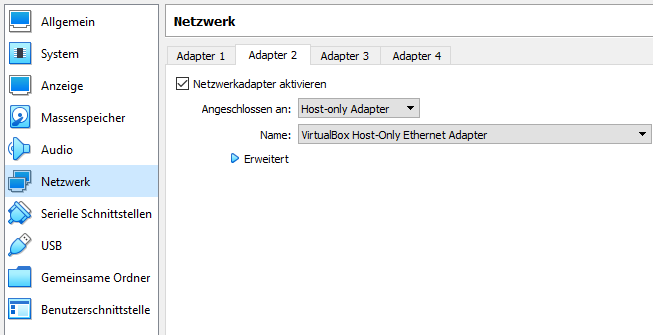
\includegraphics[scale=0.75]{images/vm-nw.png}
  \caption{Host-only Adapter}
\end{figure} \noindent
Es wird davon abgeraten ein eigenes NAT-Network zu konfigurieren, da in VirtualBox somit zwar eine Kommunikation zwischen den VMs funktioniert, jedoch keine Kommunikation zum Internet, wordurch keine Installation von WireGuard möglich ist. \newpage \noindent
Anschließend muss diesem neu angelegten Adapter eine IP-Adresse zugewiesen werden. Der Name des Adapters kann durch den Befehl \textit{ifconfig -a} identifiziert werden. Unser gewünschter Adapter ist derjenige, der keine IP Adresse besitzt. In meinem Fall war das \textit{enp0s8}. Dazu kann mit dem Befehl 
\begin{lstlisting}
$ vi /etc/network/interfaces
\end{lstlisting}
dem Adapter folgenderweise eine IP-Adresse zugewiesen werden:
\begin{lstlisting}
auto enp0s8
iface enp0s8 inet static
address 192.168.56.103
netmask 255.255.255.0
\end{lstlisting}
Zuletzt kann wieder der Befehl \textit{ifconfig} ausgeführt werden, der Folgendes zurückliefert:
\begin{figure}[H]
  \centering
  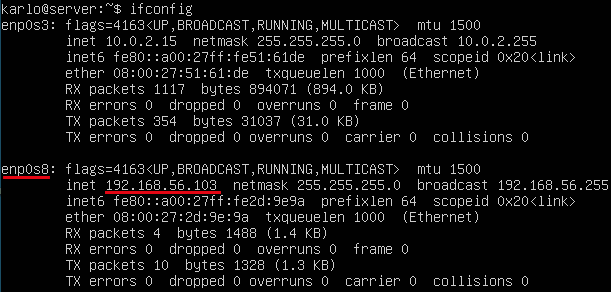
\includegraphics[scale=0.7]{images/ifconfig.PNG}
  \caption{IP Adressen der Netzwerkadapter}
\end{figure} \noindent
\subsection{Server}
Sind nun die Schritte aus Abschnitt \ref{vorbereitung} ausgeführt, kann die Installation von WireGuard beginnen. Dazu sind der Server und der Client zu starten. Um WireGuard am Server zu installieren ist am Client folgender Befehl auszuführen:
\begin{lstlisting}
$ ssh <username>@192.168.56.103
\end{lstlisting}
Anschließend wurde mit folgenden Befehlen WireGuard am Server installiert:
\begin{lstlisting}
add-apt-repository ppa:wireguard/wireguard
apt-get update
apt-get install wireguard-dkms wireguard-tools linux-headers-$(uname -r)
\end{lstlisting}
Danach wurde mit folgenden Befehlen ein private und public Key generiert:
\begin{lstlisting}
umask 077
wg genkey | tee server_private_key | wg pubkey > server_public_key
\end{lstlisting}
\newpage \noindent
Um die Konfigurationen langfristig zu speichern kann mit dem Befehl
\begin{lstlisting}
$ vi /etc/wireguard/wg0.conf
\end{lstlisting}
eine Konfigurationsdatei erstellt werden, die folgenden Inhalt enthält:
\begin{lstlisting}
[Interface]
Address = 10.100.100.1/24
SaveConfig = true
PrivateKey = 
ListenPort = 51820
PostUp = iptables -A FORWARDls -i %i -j ACCEPT; iptables -A FORWARD -o %i -j ACCEPT; iptables -t nat -A POSTROUTING -o eth0 -j MASQUERADE

PostDown = iptables -D FORWARD -i %i -j ACCEPT; iptables -D FORWARD -o %i -j ACCEPT; iptables -t nat -D POSTROUTING -o eth0 -j MASQUERADE

[Peer]
PublicKey = 
AllowedIPs = 10.100.100.2/32
\end{lstlisting}
In Zeile 4 tragen wir den generierten Private Key des Servers ein. Zeile 11 bleibt vorerst so wie sie ist. \newline\newline
Anschließend muss noch IPv4 forwarding erlaubt werden, um den Zugriff auf das gesamte LAN zu ermöglichen.
Dazu ist folgender Befehl auszuführen:
\begin{lstlisting}
$ vi /etc/sysctl.conf
\end{lstlisting}
und in folgender Zeile den Befehl:
\begin{lstlisting}
net.ipv4.ip_forward=1
\end{lstlisting}
auszukommenntieren. \newline\newline
Um diese Änderungen zu übernehmen kann entweder der Server mit dem Befehl \textit{reboot} neugestartet werden, oder mit folgenen Befehlen ohne eines Neustarts übernommen werden:
\begin{lstlisting}
sysctl -p
echo 1 > /proc/sys/net/ipv4/ip_forward
\end{lstlisting} \noindent
Soweit so gut. Der Server ist nun konfiguriert. \newline\newline
WireGuard kann nun mit folgenden Befehl gestartet werden:
\begin{lstlisting}
$ wg-quick up wg0
\end{lstlisting}
Möchte man, dass WireGuard automatisch gestartet wird, sobald der Server gestartet wird, kann man das mit folgenden Befehl erreichen:
\begin{lstlisting}
$ systemctl enable wg-quick@wg0.service 
\end{lstlisting}
\newpage
\subsection{Client}
Zuerst muss WireGuard installiert werden. Dieser Vorgang ist in Abschnitt \ref{installation} erklärt. Für Ubuntu 19.10 habe ich folgenden Befehl ausgeführt:
\begin{lstlisting}
$ sudo apt install wireguard
\end{lstlisting} 
 Anschließend wird für den Client ein private und public Key generiert.
\begin{lstlisting}
wg genkey | tee client_private_key | wg pubkey > client_public_key
\end{lstlisting}
Nun muss noch in der Server Konfigurationsdatei in Zeile 11 der Public Key des Clients eingetragen werden. \newline\newline
Zuletzt wird wieder eine Konfigurationsdatei angelegt.
\begin{lstlisting}
$ vi /etc/wireguard/wg0-client.conf
\end{lstlisting}
Diese hat folgenden Inhalt:
\begin{lstlisting}
[Interface]
Address = 10.100.100.2/32
PrivateKey =

[Peer]
PublicKey =
Endpoint = :51820
AllowedIPs = 0.0.0.0/0
PersistentKeepalive = 21
\end{lstlisting}
In Zeile 3 wird der Private Key des Clients eingetragen und in Zeile 6 der Public Key des Servers. Zeile 7 enthält zusätzlich noch die IP Adresse des Servers. \newline
Wireguard ist nun am Client konfiguriert und kann mit folgenden Befehl gestartet werden:
\begin{lstlisting}
$ sudo wg-quick up wg0-client
\end{lstlisting}
Überprüft man nun die IP Adresse des Clients, stellt man fest, dass die IP Adresse des WireGuard Servers zu sehen ist, anstelle der ursprünglichen IP Adresse des Clients. Das bedeutet, dass die IP Adresse des Clients nun nicht mehr öffentlich sichtbar ist und unser VPN Server korrekt funktioniert. Näher wird darauf in Abschnitt 1.4.1 eingegangen. \newline \newline
Führt man den Befehl
\begin{lstlisting}
$ sudo wg-quick down wg0-client
\end{lstlisting}
aus erhält man wieder die ursprüngliche IP Adresse des Clients.
\newpage
\section{Technische Funktionalität} % Foto einfügen von VPN Tunneling? (von ko skripten)
\subsection{VPN}
Als VPN (Virtual Private Network) bezeichnet man ein logisches privates Netzwerk, das auf einer öffentlichen Infrastruktur zugänglich ist. Ausschließlich Kommunikationspartner, die zu diesem privaten Netzwerk gehören, können miteinander kommunizieren.\newline
Die Grundsätze von VPNs um eine sichere Kommunikation zu gewährleisten lauten:
\begin{itemize}
    \item \textbf{Authentizität} \newline
    Eigenschaft, die gewährleistet, dass ein Kommunikationspartner tatsächlich derjenige ist, der er vorgibt zu sein.
    \item \textbf{Vertraulichkeit} \newline
    Schutz vor unbefugter Preisgabe von Information. Vertrauliche Daten dürfen ausschließlich den Kommunikationspartnern im privaten Netzwerk zugänglich sein.
    \item \textbf{Integrität} \newline
    Sicherstellung der Korrektheit von Daten.
\end{itemize}
\begin{figure}[H]
  \centering
  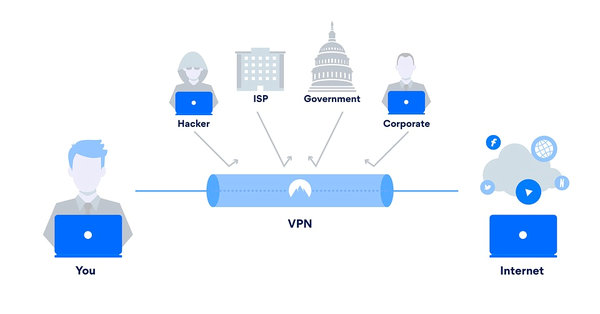
\includegraphics[scale=0.85]{images/vpn.jpg}
  \caption{VPN Funktionsweise}
\end{figure}
\subsubsection{Ablauf VPN-Verbindung}
\begin{enumerate}
    \item Ein VPN-Client stellt eine Verbindung zu einem VPN-Server über ein VPN-Protokoll her.
    \item Der VPN-Server überprüft die Zugangsdaten, nimmt die Verbindung dementsprechend an und einigt sich mit dem VPN-Client auf einen Schlüssel zur sicheren Kommunikation.
    \item Es entsteht eine verschlüsselte Verbindung zwischen dem VPN-Server und dem VPN-Client, die auch als \textit{Tunnel} bezeichnet wird und eine physische Verbindung simuliert.
    \item Der VPN-Client kann auf das lokale Netzwerk des VPN Servers zugreifen, als wäre er vor Ort mit diesem Netzwerk verbunden.
\end{enumerate}
\newpage
\noindent
\section{Wireguard}
WireGuard arbeitet ausschließlich auf der 3. Schicht des OSI Modells und bietet eine Unterstützung für IPv4 und IPv6. Zur Übertragung der verschlüsselten IP-Pakete wird UDP verwendet.
\begin{figure}[H]
  \centering
  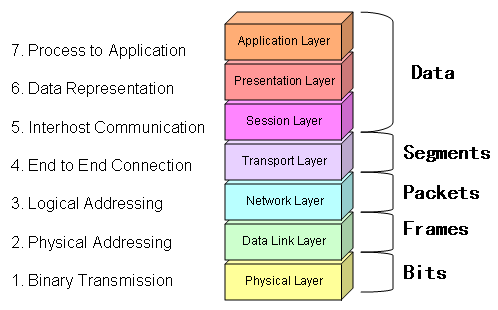
\includegraphics[scale=0.65]{images/osi.PNG}
  \caption{Osi Modell}
\end{figure}\noindent
Vorteile:
\begin{itemize}
    \item einfache Nutzbarkeit
    \item minimale Codebasis
    \item Open Source
    \item moderne Kryptographietechniken
    \item Unterstützung vieler Betriebssysteme
    \item schneller Verbindungsaufbau
    \item schnelle Geschwindigkeit \newline
    
\end{itemize}
Um ein hohes Sicherheitsniveau bei der Verschlüsselung der Daten zu erreichen, nutzt WireGuard moderne kryptographische Verfahren:
\begin{itemize}
    \item Curve25519 zum Schlüsselaustausch im Handshake mit Elliptic Curve Diffie-Hellman (ECDH)
    \item ChaCha20 und Poly1305 für die symmetrische Verschlüsselung und den Austausch der Daten
    \item BLAKE2s für die Hashfunktion
    \item Ed25519 für die Zertifikate
\end{itemize}
\newpage \noindent
Die Identität der VPN-Teilnehmer ist an ihren öffentlichen Schlüssel geknüpft. Damit können sich die Peers untereinander authentifizieren. WireGuard basiert auf einem Konzept namens \textit{Cryptokey-Routing}. Dabei ist für jeden Peer eine Tabelle mit den public Keys und Allowed IPs seiner Gegenstellen enthalten. Daraus leitet WireGuard eine interne Routing-Tabelle ab, die den Weg für jedes Paket kennt. Verbindungen werden ähnlich wie bei SSH durch den Austausch der öffentlichen Schlüssel aufgebaut. Dabei setzt WireGuard nicht auf eine klassische Client-Server Architektur, sondern erzeugt ein Peer-to-Peer Netzwerk. Die Verbindung zwischen zwei Peers realisiert WireGuard über einen einzelnen, frei wählbaren UDP-Port. Wird kein Port angegeben, beginnt WireGuard bei 51820/UDP.
\begin{figure}[H]
  \centering
  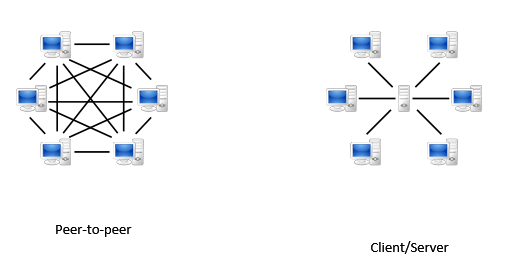
\includegraphics[scale=0.75]{images/peer2peer.png}
  \caption{Peer to Peer vs. Client/Server Architektur}
\end{figure} 
\noindent Beispiel für Verschlüsseln eines Pakets:
\begin{enumerate}
    \item Es soll ein Paket an die IP Adresse 192.168.30.8 geschickt werden. WireGuard überprüft, welchem Peer diese IP Adresse entspricht. 
    \item Wird dieser Vorgang erfolgreich durchgeführt, erfolgt eine Verschlüsselung des IP Pakets mit dessen Public Key. Sonst wird das Paket verworfen.
    \item WireGuard überprüft den öffentlichen Endpoint von diesem Client. Dieser ist beispielsweise Port 53133 mit 216.58.211.110.
    \item Das verschlüsselte Paket aus Punkt 2 wird nun an den Endpoint 216.58.211.110:53133 durch UDP weitergeleitet.\newline
\end{enumerate}
Beispiel für Entschlüsseln eines Pakets:
\begin{enumerate}
    \item Empfängt ein WireGuard Peer ein Paket, wird dieses durch den eigenen private Key entschlüsselt.
    \item Wird dieser Vorgang erfolgreich durchgeführt und für einen bekannten Peer X authentifiziert, wird sein letzter öffentlicher Endpoint ermittelt.
    \item Das entschlüsselte Paket enthält das Klartext Paket von der IP Adresse 192.168.43.89. Nun wird geprüft, ob der Peer X diesem Peer Pakete der IP Adresse 192.168.43.89 schicken darf. 
    \item Wenn die Prüfung erfolgreich ist, wird das Paket akzeptiert. Sonst wird das Paket verworfen.

\end{enumerate}
\newpage \noindent
Performance Tests (Abbildung \ref{performance}) zeigen, dass WireGuard wesentlich leistungsfähiger als die Konkurrenten IPsec und OpenVPN abschließt. Im Gegensatz zu diesen Protokollen, welche hunderttausende LOC haben, enthält WireGuard bloß 4000 Zeilen. Dies ist aus zwei Gründen ein großer Sicherheits Vorteil: Zum einen enthält weniger Code auch potenziell weniger Fehler. Zum anderen sind dadurch potentielle Schwachstellen schneller zu finden. Einen weiteren Performance Schub bekommt WireGuard dadurch, dass die Software serverseitig als Linux-Kernelmodul ausgeführt wird.
Außerdem wurde WireGuard unter der GPLv2 Lizenz veröffentlicht und ist somit kostenlos einsetzbar.
\begin{figure}[H]
  \centering
  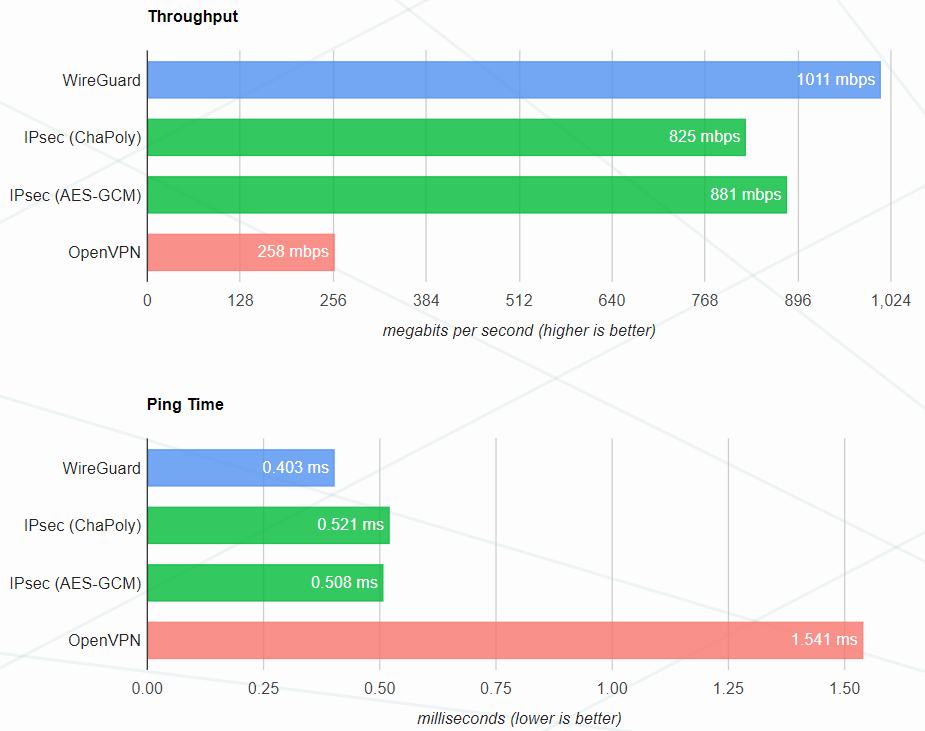
\includegraphics[scale=0.65]{images/performance.PNG}
  \caption{WireGuard Performancevergleich}
  \label{performance}
\end{figure}

Nachteile:
\begin{itemize}
    \item experimentelle Entwicklung \newline
    Obwohl WireGuard schon benutzbar ist, ist die Entwicklung einer stabilen Version noch nicht abgeschlossen und muss noch Sicherheitsaudits durchlaufen, in denen Experten die Codequalität überprüfen.
    \item eingeschränkte Anonymität \newline
    WireGuard unterstützt keine dynamische Adressverwaltung, wodurch dem Client im Vorhinein eine vordefinierte IP Adresse zugewiesen werden muss, welche auf jedem Server mit dem entsprechenden Schlüssel verknüpft ist.
\end{itemize}
\newpage
\section{Docker}
In der heutigen Zeit möchte man Software zwischen unterschiedlichen Plattformen und
Infrastrukturen bewegen, ohne ständig die Vorraussetzungen für das Deployment und den Betrieb
anzupassen.\newline
Docker gibt uns die Möglichkeit mithilfe von Container-Technologie, Anwendungen in
verschiedensten Umgebungen mit den unterschiedlichsten Vorraussetzungen auszuführen, ohne
dafür das komplette System virtualisieren zu müssen.
\section{Vorteile}
Die Plattform bietet die Möglichkeit unsere Applikation in eine isolierte Umgebung zu verpacken,
gennant \textit{Container}. Container benötigen weit weniger Ressourcen als z.B. eine Virtuelle
Maschine. Warum dies so ist, wird in der Erklärung der Container-Technologie näher erläutert.
Diese Umgebung verändert sich nicht, was bedeutet, dass keine Inkonsistenzen auftreten und die
Applikation immer in der exakt gleichen Umgebung läuft.
Docker ist somit durch seine Container-Technologie im Hinblick auf Systemressourcen weitaus
effizienter und modularer als eine Virtuelle Maschine.
\subsection{Container Technologie}
Docker basiert auf der Container-Technologie. Die Grafik \ref{contTech} vergleicht eine Virtuelle Maschine mit
einer Container Engine. Bei einer virtuellen Maschine wird ein Hypervisor benötigt, auf welchem die VMs laufen. In einer VM wird das gesamte Betriebssystem virtualisiert und auf diesem Betriebssystem läuft dann
unsere Applikation. Die Container Technologie funktioniert so, dass auf dem Host Betriebssystem eine sogenannte
Container Engine läuft (in unserem Fall die Docker Engine), auf der sich wiederum die Container
befinden. Anstatt also die komplette Hardware zu virtualisieren, wie es bei VMs der Fall ist, werden bei
einem Docker Container nur die benötigten Binaries/Libraries virtualisiert, welche für die
Anwendung, die am Container laufen soll, benötigt werden.

\begin{figure}[H]
  \centering
  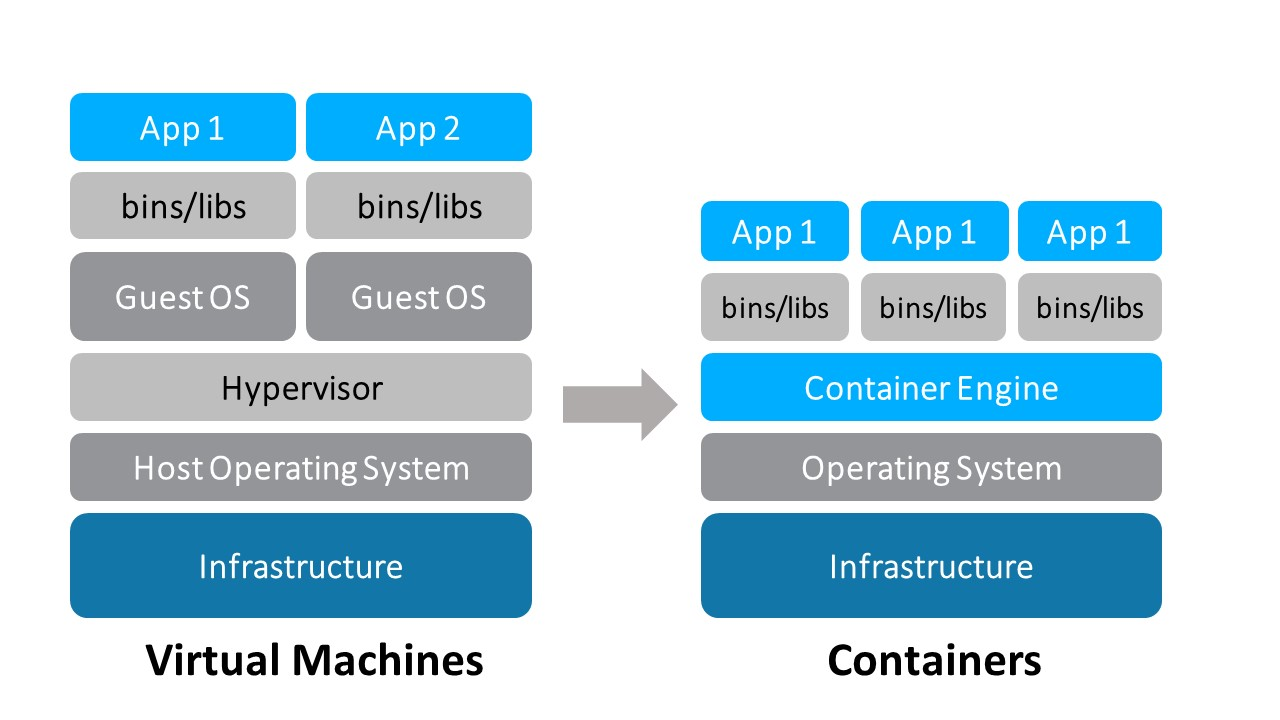
\includegraphics[scale=0.35]{images/containertech.jpg}
  \caption{Docker vs VM}
  \label{contTech}
\end{figure}
\subsection{Image}
Ein Image ist ein Template mit verschiedenen Konfigurationen für einen Container. Meist basiert
ein Image auf einem anderen, enthält jedoch zusätzliche Anpassungen.
Ein Image wird durch ein sogenanntes “Dockerfile” dargestellt.
\subsection{Container}
Ein Container ist eine Instanz eines Images.

\begin{figure}[H]
  \centering
  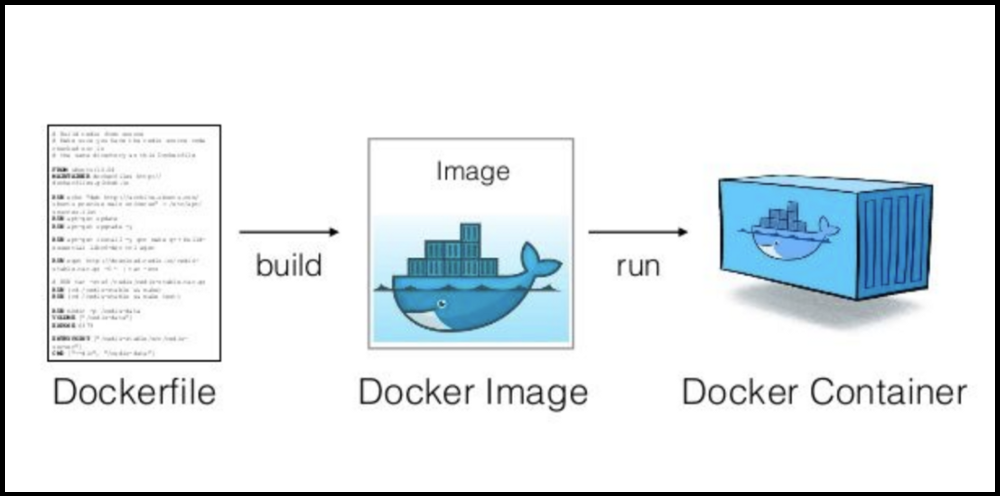
\includegraphics[scale=0.35]{images/docker.PNG}
  \caption{Docker Build Prozess}
  \label{performance}
\end{figure}

\section{Einsatz im Container}
Es besteht die Möglichkeit WireGuard in einem Docker Container zu verwenden. In den folgenden Schritten wird dieser Vorgang erklärt:
\begin{enumerate}
    \item \href{https://docs.docker.com/docker-for-windows/install/}{Docker} installieren
    \item docker-compose Datei erstellen \newline
    \begin{lstlisting}
    version: "2"
    services:
     vpn:
      image: cmulk/wireguard-docker:buster
      volumes:
       - data:/etc/wireguard
      networks:
       - net
      ports:
       - 5555:5555/udp
      restart: unless-stopped
      cap_add:
       - NET_ADMIN
       - SYS_MODULE
    
    networks:
      net:
    
    volumes:
     data:
      driver: local
    \end{lstlisting}
    \item Projekt builden
    \begin{lstlisting}
    git clone https://github.com/cmulk/wireguard-docker.git
    cd wireguard-docker
    git checkout stretch 
    
    docker build -t wireguard:local .
    \end{lstlisting}
    \item Projekt zum 1. Mal ausführen
    \begin{lstlisting}
    docker run -it --rm --cap-add sys_module -v /lib/modules:/lib/modules cmulk/wireguard-docker:buster install-module 
    \end{lstlisting}
\end{enumerate}
Nach dem das Projekt bereits einmal ausgeführt wurde, erfolgt dies für die nächsten Runs mit dem Befehl:
\begin{lstlisting}
docker run --cap-add net_admin --cap-add sys_module -v <config volume or host dir>:/etc/wireguard -p <externalport>:<dockerport>/udp cmulk/wireguard-docker:buster
\end{lstlisting}

